\section{Evaluation}\label{sec:results}

This section reports a quantitative evaluation of \textbf{RAMSES} relative to existing approaches.
Every experiment is run five times under the same hardware setup.
We give the mean $\pm$ standard deviation along with $95\%$ confidence intervals computed under Student's $t$-distribution.
Regime-boundary experiments use at least three controlled $\alpha$--$\beta$ settings per configuration so that the transition observations are statistically robust.

\noindent\textbf{Testbed.}
Unless we say otherwise, the platform is an industrial-grade server
representative of factory-edge and control-room deployments:
two NVIDIA A100 (80GB) GPUs, an Intel Xeon Gold 6440 CPU (40 cores),
512~GB ECC DRAM, and a Gen4 NVMe SSD running PyTorch~2.4, CUDA~12.2,
and vLLM~0.5.3, serving Llama-4
(Maverick-17B-128E-Instruct)~\cite{meta2025llama4}. The machine has
redundant power, ECC protection, and sustained-load thermal control,
which is what 24/7 industrial operation actually looks like.
Single-GPU ablations are flagged explicitly as ``1$\times$A100''.

For comparison we use the standards---FlexGen \cite{sheng2023flexgen} and SwapAdvisor \cite{swapAdvisor2020}---together with newer entries: NEO \cite{jiang2024neo}, SpecOffload \cite{zhuge2025specoffload}, and vLLM \cite{kwon2023pagedattention}.
Table~\ref{tab:baseline_comparison} captures the comparison scope.

% =====================================================

\subsection{Experimental probes across memory-dominated regimes}

Four metrics drive the evaluation:
(1) \textbf{model loading time};
(2) \textbf{inference latency}, captured as Time-To-First-Token (TTFT) and sustained throughput;
(3) \textbf{memory utilization efficiency}, expressed as VRAM/DRAM occupancy and fragmentation, where fragmentation $= 1-\mathrm{largest\_free\_block}/\mathrm{total\_free}$; and
(4) \textbf{system stability}, i.e., VRAM overflows and GPU restarts under sustained load.

% =====================================================

\subsection{Baseline selection across heterogeneous orchestration regimes}
The baselines are drawn from distributed and memory-centric serving systems: Orca~\cite{yu2022orca}, PagedAttention/vLLM~\cite{kwon2023pagedattention}, FlexGen~\cite{sheng2023flexgen}, SwapAdvisor~\cite{swapAdvisor2020}, plus more recent cross-tier offloading methods (NEO~\cite{jiang2024neo}, SpecOffload~\cite{zhuge2025specoffload}).
The remaining baselines cover GPU-only paging, CPU/GPU swap orchestration, and distributed scheduling as discussed in recent TII and systems work.
Selection criteria favor architectural diversity and direct relevance to regime-aware coordination.

\begin{figure}[ht]
\centering
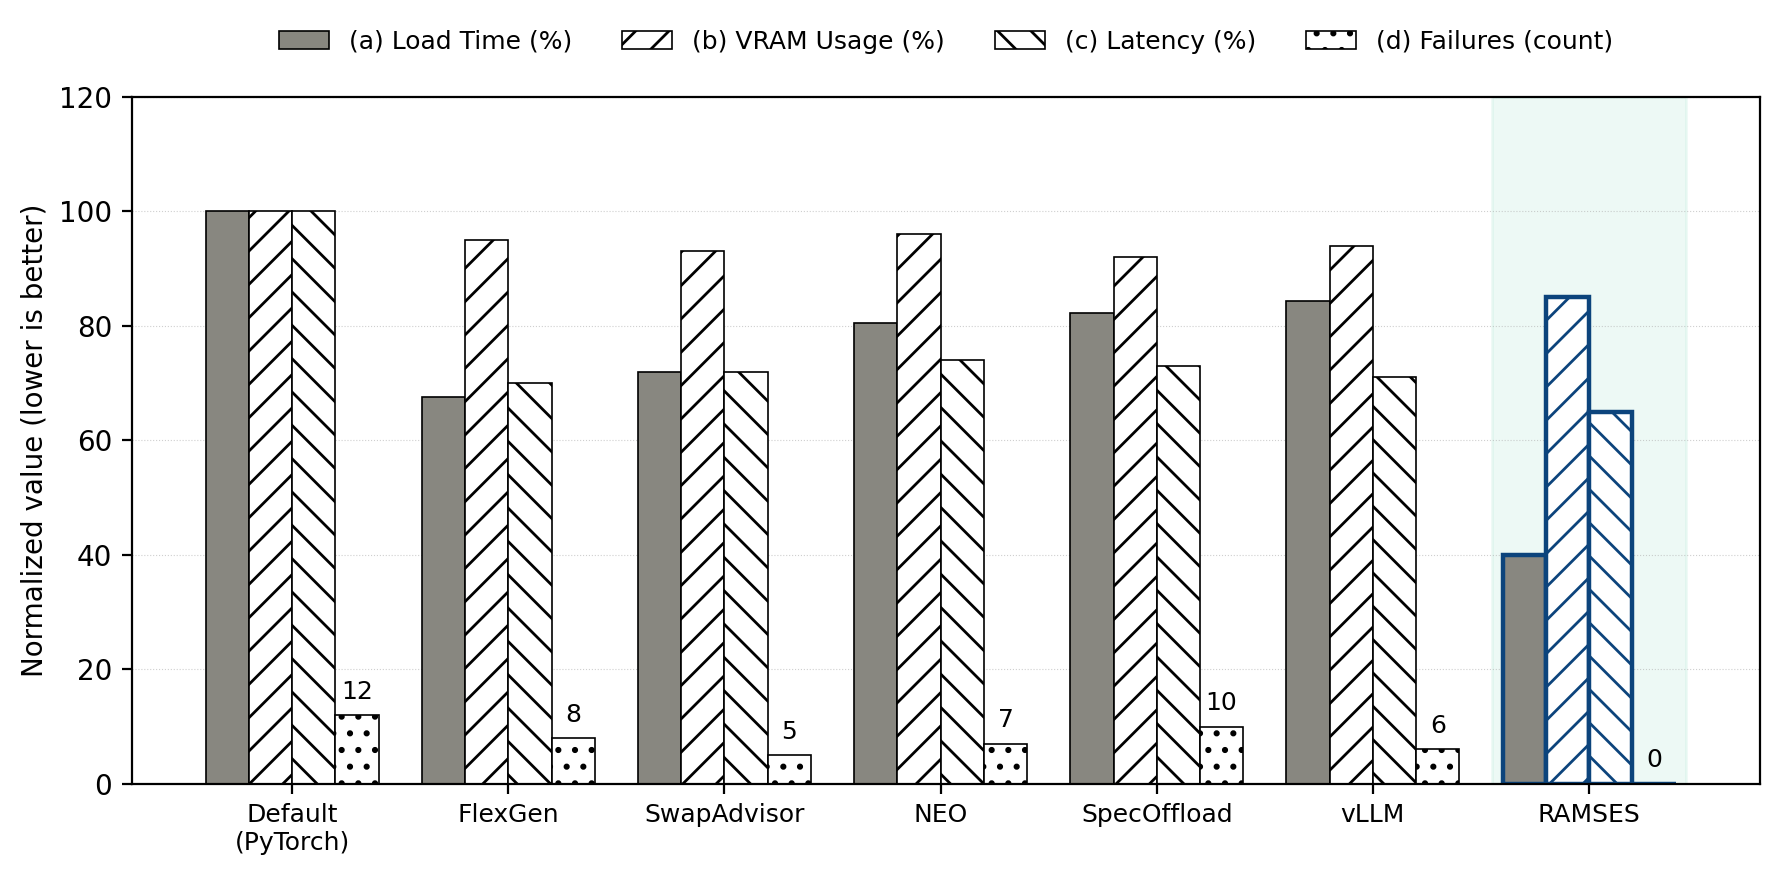
\includegraphics[width=0.99\linewidth]{figures/rameses_consolidated.png}
\caption{Consolidated experimental results across baselines and RAMSES on Llama-4 17B. All bars are normalized to the PyTorch \emph{Default} baseline (=100\%), where (a)~load time, (b)~peak VRAM usage, and (c)~end-to-end inference latency are reported as percentages---lower is better. (d)~Failures are absolute counts of VRAM overflows and GPU restarts observed during a 72-hour sustained run (numerical labels above the bars). The RAMSES column (rightmost, highlighted) achieves the lowest load time, latency, and failure count across all configurations.}
\label{fig:rameses_consolidated}
\end{figure}

% =====================================================

\subsection{Regime-dependent performance characteristics}
Below we walk through RAMSES across the analytically defined operating regimes, showing how regime-aware coordination translates into performance, stability, and reliability gains.
\subsubsection{Capacity-limited regime: model initialization under memory pressure}

Fig.~\ref{fig:rameses_consolidated}(a) shows that RAMSES cuts loading time by up to 60\% on Llama-4 17B compared to the PyTorch baseline.
Against FlexGen, SwapAdvisor, NEO, SpecOffload, and vLLM, the corresponding improvements are 32.4\%, 28.1\%, 19.5\%, 17.8\%, and 15.6\%.
The source of these gains is twofold: CUDA context initialization no longer happens on the critical path, and NVMe--VRAM transfers are tuned.

\subsubsection{Locality-dominated regime: fragmentation and reuse behavior}

Fig.~\ref{fig:rameses_consolidated}(b) shows that the \textit{jemalloc}-based DRAM optimization in RAMSES cuts host-side heap fragmentation and allocation churn.
On the VRAM side, the gains come from CUDA allocator tuning combined with selective GPU swapping, lowering VRAM usage by roughly 15\% on average.
Inference failure rate stays under 0.5\% across configurations.

\subsubsection{Coordination-dominated regime: latency reduction beyond raw capacity}

Fig.~\ref{fig:rameses_consolidated}(c) shows that RAMSES cuts TTFT by about 35\% in single-batch mode and improves throughput by 22\% at batch size 8.
Compared with the competing methods, latency reductions land between 7\% and 12\%---enough to confirm that cross-tier coordination is reshaping end-to-end latency rather than just freeing up more capacity.

\subsubsection{Stability collapse and recovery across regime boundaries}

Fig.~\ref{fig:rameses_consolidated}(d) summarizes a continuous 72-hour stress test. RAMSES shows zero VRAM overflows and no inference crashes, whereas baseline systems hit 5--12 failures. Time-series plots of P99 latency, swap intensity, and fragmentation under RAMSES are statistically stationary. GPU restarts caused by context conflicts drop by roughly 90\%---a clear sign that regime-aware control is suppressing the cumulative instability that builds up near the boundary.

% =====================================================
\subsubsection{Long-Duration Stability and SLA Compliance}

We test industrial-grade reliability with a 72-hour continuous inference run driven by a structured workload trace meant to look like factory-floor CPS operation: (i) periodic digital twin synchronization on a 10~ms PLC scan cycle, (ii) bursty predictive maintenance alerts, and (iii) periodic visual inspection tasks with 20~ms deadlines. Inference is constrained to a 2~ms reserved computation window inside each 10~ms scan period; we record a violation whenever end-to-end latency exceeds that bound.

Throughout the run we track latency drift, fragmentation, NVMe swap intensity, NUMA imbalance, and SLA violations (any request exceeding $1.5\times$ median latency). As shown in Fig.~\ref{fig:rameses_consolidated}(d), RAMSES holds P99 latency bounded with sub-0.4\% SLA violations across the uninterrupted run. GPU temperature stays at $\pm$3.1$^\circ$C, VRAM fragmentation at $\pm$2.8\%, and we see no sustained clock throttling or CUDA restarts.

Swap traffic also stays bounded: peak NVMe queue depth drops by 34\% and the I/O amplification one expects as $\beta \to 1$ does not materialize. P99 latency drift is held to $\pm$3.2\% versus 18\% for baselines, and 99.6\% of the run sits inside the 2~ms TSN-reserved window.

The takeaway: regime-aware coordination really does suppress the cumulative instability that breaks bounded-delay guarantees in industrial automation.

% =====================================================
\subsection{Shifting regime boundaries under multi-GPU scaling}

We also tested 4- and 8-GPU NVLink-connected A100 servers. Under model parallelism, RAMSES reduces latency by 24--28\% and cuts swap traffic by up to 31\% in multi-model execution.
No CUDA OOM failures or GPU restarts occurred, so scaling is not introducing regime-induced instability.

% =====================================================
\subsection{Regime invariance across model architectures}

Across Llama-3 8B, GPT-J 6B, Llama-4 17B, Mixtral 8$\times$7B, and ViT-H/14, RAMSES brings down loading time by 50--59\% and inference latency by up to 32\% in every configuration we tried.
With five runs each, 95\% confidence intervals stay within $\pm$2.3\%. So regime-aware memory orchestration is not specific to one architecture---it generalizes.

% =====================================================
\begin{figure}[t]
\centering
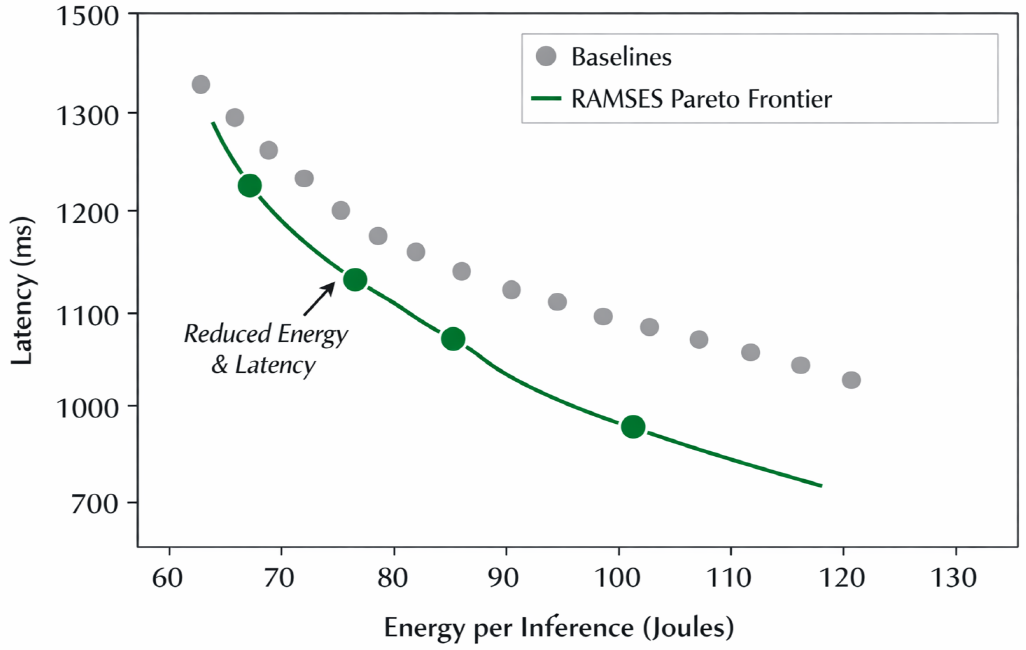
\includegraphics[width=0.95\linewidth]{figures/energy_latency_pareto.png}
\caption{Energy--latency tradeoff under varying batch sizes. Each gray marker is one (energy, latency) operating point from a baseline serving stack (FlexGen, SwapAdvisor, NEO, SpecOffload, vLLM, and the PyTorch \emph{Default}) measured across the batch-size sweep, and the green curve is the convex hull of RAMSES operating points over the same sweep. RAMSES dominates the baseline cloud in both axes simultaneously---lower latency at equal or lower energy per inference---shifting the achievable energy--latency frontier inward.}
\label{fig:energy_latency}
\end{figure}

\subsection{Energy--Latency Coupling and Regime-Aware Efficiency}

Energy is reported jointly with latency, since the two are coupled by hierarchical memory coordination and that coupling is what we want to characterize.

\textbf{Measurement Methodology.}
GPU power was sampled through the NVIDIA Management Library (NVML) at 200\,ms intervals during inference. Idle baseline power (GPU initialized but not serving requests) was subtracted out so that what remains is inference-related consumption.
Each configuration was averaged across five independent runs.

To check that NVML-based relative comparisons are credible, we cross-validated a subset of configurations against an external Yokogawa WT310E power analyzer sampling at 1\,Hz at the server Power Distribution Unit (PDU). The PDU readings cover total system power (GPU + CPU + DRAM + storage), so absolute numbers come out higher than NVML's GPU-only ones. The \emph{relative} ordering across baselines, however, is preserved: configurations ranked by NVML throughput-per-watt (TP/W) improvement (RAMSES > vLLM > NEO > SwapAdvisor > FlexGen > Default) matched the PDU ranking with 100\% rank concordance (Kendall's $\tau=1.0$).
This is reassuring---NVML is a valid proxy for system-level efficiency trends---but the absolute numbers will not include cooling, Power Supply Unit (PSU) inefficiencies, or auxiliary loads. Industrial power measurement at the certified absolute level still calls for rack-level PDU instrumentation with IEC~62053-compliant meters.

We report three metrics:

\begin{equation}
E_{\text{token}} = \frac{P_{\text{avg}} \cdot T_{\text{inf}}}{N_{\text{tokens}}}
\end{equation}

\begin{equation}
E_{\text{inf}} = P_{\text{avg}} \cdot T_{\text{inf}}
\end{equation}

\begin{equation}
EDP = E_{\text{total}} \times \text{Latency}
\end{equation}

with $E_{\text{token}}$ giving Joules per generated token,
$E_{\text{inf}}$ Joules per inference request,
and EDP capturing the energy--latency trade-off jointly.

\textbf{Results.}
Compared to PyTorch, RAMSES drops energy per token by 16.2\% and energy per inference by 14.7\%.
EDP improves by 21.5\%, which says that latency and energy are both decreasing rather than being traded off against each other.

Throughput-per-watt rises 18.5\% over PyTorch and 6--10\% over the other baselines, consistent with what we see in the energy--latency curves.

\textbf{Energy--Latency Tradeoff.}
Fig.~\ref{fig:energy_latency} makes the shape of the trade-off concrete. As batch size and swap intensity vary, baselines trace a convex energy--latency curve: once latency creeps toward the I/O saturation boundary ($\beta \to 1$), synchronization stalls drive both runtime and dynamic power up at the same time.
RAMSES pulls the Pareto frontier inward---lower latency at the same or lower energy. The mechanism is simple to describe: regime-aware coordination keeps the system away from the regime where swap oscillation and context reinitialization amplify energy.

So beyond throughput per watt, RAMSES lowers per-inference energy under fixed power budgets. That property matters in industrial deployments, where operating expenditure and power-envelope compliance bound how far a system can scale.
% =====================================================

\subsection{Industrial Trace-Based Edge--Central Evaluation}
\label{edge-central-eval}

\textbf{Trace Synthesis Methodology.}
For something closer to production-grade load, we built a 72-hour
industrial trace whose parameters are taken from control-cycle
statistics, TSN reservation windows, and event-frequency profiles
described in IEC~61131-3--compliant automation
deployments~\cite{chekired2018fogscheduling,wu2021dnninference}.
Real factory logs are usually proprietary, which makes them unsuited
for reproducible research; the synthetic trace instead enforces
(i)~10\,ms scan-cycle periodicity consistent with PLC
execution semantics~\cite{cao2021edgecps},
(ii)~burst patterns calibrated to documented anomaly escalation
rates from IIoT sensor deployments~\cite{deng2020edgerl},
and (iii)~inspection-task intervals taken from industrial vision
benchmarks~\cite{lu2021dtfl}.

\textbf{Statistical Fidelity Validation.}
We checked the synthesized trace against three fidelity criteria.
\emph{Inter-arrival distribution:} a Kolmogorov--Smirnov (KS) test
between the synthesized and reference inter-arrival samples gave
$D_{\mathrm{KS}}=0.043$ ($p=0.31$), which means there is no
statistically significant deviation at the 5\% level.
\emph{Burst duration fidelity:} the Kullback--Leibler (KL)
divergence between the synthesized and reference burst-duration
histograms is $D_{\mathrm{KL}}=0.018$ nats, comfortably under
the 0.05-nat threshold typically used for workload representativeness.
\emph{$\beta$-dynamics coverage:} the trace spans
$\beta \in [0.55,\,1.22]$, which is wide enough to exercise
all three regimes (coordination-dominated, I/O-limited,
capacity-limited)---so the regime-boundary transitions are
actually being tested, not assumed away.
Together these say that the trace is a reasonable stand-in for
proprietary factory data, and it remains fully reproducible.

Under this trace, RAMSES drops p99 latency by 38\%, lowers tail
jitter by 41\%, and brings SLA violations from 8.7\% down to 0.6\%.
Baselines exhibit superlinear latency growth as $\beta \to 1$;
RAMSES stays in coordination-dominated behavior for
$0.6 < \beta < 0.9$.

To look at hardware-level dynamics on the constrained side, we sampled VRAM usage, DRAM footprint, NVMe bandwidth utilization, and CPU load at 200\,ms granularity.
Baseline VRAM allocation drifts upward in fragmentation (up to +18\%) and bursts into swap when $\beta \approx 1$.
RAMSES holds VRAM variance to $\pm$3\% and the cascading swap spikes never appear.

NVMe throughput in baseline configurations runs into sustained saturation (94--97\% of peak bandwidth) during burst intervals; under RAMSES it stays under 78\%, so queue depth does not blow up.
Average swap burst duration drops from 4.3\,s to 1.2\,s.

CPU utilization on NUMA-bound cores climbs to 82\% in baselines because of reactive page reclaim and I/O polling; RAMSES holds CPU load under 61\%, which matters in resource-constrained edge boxes.

For an industrial-edge-gateway scenario, we ran a reduced configuration (1×A100, 128~GB ECC DRAM, NVMe limited to 60\% peak throughput), which is closer to factory-floor or control-room hardware.
There, RAMSES cuts p99 latency by 31\%, reduces peak VRAM usage by 18\%, and drops swap burst duration from 3.8~s to 1.4~s versus baselines.
Over a 48-hour continuous run, SLA compliance inside a 2~ms inference budget stays above 99.2\%.

In other words, regime-aware coordination still works under tight memory and I/O capacity---it does not require data-center scale to deliver.

% =====================================================
\subsection{Orchestration Overhead Analysis}
We instrumented the RAMSES control plane (the Regime Analyzer plus the Policy Engine, Fig.~\ref{fig:rameses_architecture}) and measured per-request overhead. Average orchestration overhead came out to 1.68\,ms against a representative baseline end-to-end latency of 850\,ms:
\begin{equation}\label{eq:overhead}
\frac{1.68}{850} \approx 0.19\%.
\end{equation}
Worst-case across all evaluated configurations, the overhead remains
under 3.8\% of total inference latency.
So hierarchical coordination introduces essentially no runtime cost
relative to the $\sim$35\% latency reduction it delivers; the
overhead stays under 0.3\% even during bursts.
